\documentclass[a4paper, 12pt]{article}
%\documentclass{book}

% Important Packages:
 \usepackage{amsmath}    % need for subequations
 \usepackage{amsfonts}
 \usepackage{amsthm}
 \usepackage{graphicx}   % need for figures
 \usepackage{verbatim}   % useful for program listings
 %\usepackage{subfig}  % use for side-by-side figures
 %\usepackage{wrapfig}
 %\usepackage{listings}	 % creates code blocks
 %\usepackage[colorlinks=true]{hyperref}   % use for hypertext links, including
                     % those to external documents and URLs
 %\usepackage{multirow}
 %\usepackage{tikz}
 %\usepackage{enumerate}
 %\usetikzlibrary{decorations.pathreplacing,decorations.pathmorphing}
 %\usetikzlibrary{calc}
 %\usepackage[colorinlistoftodos]{todonotes}
 
 % Useful macros 
 \def\tcb#1{\color{blue}{#1}}
 \def\tcr#1{\color{red}{#1}}	
 \def\tcg#1{\color{green}{#1}}
 \def\be{\begin{eqnarray}}	 	\def\ee{\end{eqnarray}}
 \def\bea{\begin{eqnarray}}	 	\def\eea{\end{eqnarray}}
 \def\bean{\begin{eqnarray*}}	\def\eean{\end{eqnarray*}}
 
 \def\D{\displaystyle}
 \def\T{\textstyle}
 \def\l{\left}
 \def\r{\right}
 \def\nf{n_{\!f}} % quark flavours
 \def\pa{\partial}
 \def\eg{e.\,g.}
 \def\ie{i.\,e.}

 \def\be{\begin{equation}}
 \def\ee{\end{equation}}
 \def\bea{\begin{eqnarray}}
 \def\eea{\end{eqnarray}}
 \def\bean{\begin{eqnarray*}}
 \def\eean{\end{eqnarray*}}
 \def\gsim{\mathrel{\rlap{\lower0.2em\hbox{$\sim$}}\raise0.2em\hbox{$>$}}}
 \def\ksim{\mathrel{\rlap{\lower0.2em\hbox{$\sim$}}\raise0.2em\hbox{$<$}}}
 \def\kg{\mathrel{\rlap{\lower0.25em\hbox{$>$}}\raise0.25em\hbox{$<$}}}
 
 \def\AA{${\buildrel_{\circ} \over {\mathrm{A}}}$}
 \def\bm#1{\mbox{\boldmath$#1$}}
 \newcommand{\eq}[1]{(\ref{#1})} 
 \def\pd{\partial}
 \def\d{\textrm{d}} 
 \def\T{\textstyle}
 \def\eg{e.\,g.}	% exempli gratia (for the sake of example)
 \def\ie{i.\,e.}	% id est (that is)


 % Page configuration:
 \topmargin -2.0cm
 \oddsidemargin -0.85cm
 \evensidemargin -0.85cm
 \textwidth 18cm
 \textheight 24cm
 
\begin{document}
\begin{center}
\textbf{Stellenbosch Camp December 2017 \\ Senior Test 2} \\
\textbf{Solutions}
\end{center}

\begin{enumerate}
    % EGMO 2013 solutions: https://www.egmo.org/egmos/egmo2/solutions.pdf

    % QUESTION 1
    \item[1.] Letting $x = y = 0$ yields $f(0) = 0$. For $y = 0$, we obtain $f(x^2) = x^2$ which implies $f(x) = x$ for all $x \geq 0$. For $x = 0$, we obtain $f(-y^2) = -f(y^2) = -y^2$, which implies $f(x) = x$ for all $x \leq 0$. Hence $f(x) = x$ for all $x \in \mathbb{R}$ which can easily be checked to be a solution.
    
    \item[2.] 
    
    % EGMO 2012 Q1
    \item[3.] Let $l_C$ be the tangent at $C$ to the circumcircle of $\triangle ABC$. As $CO \perp l_C$, the lines $DE$ and $l_C$ are parallel. Now we find that
    $$ \angle CDE = \angle (BC, l_C) = \angle BAC $$
    hence the quadrilateral $BDEA$ is cyclic. Analogously, we find that the quadrilateral $CDFA$ is cyclic. As we now have $\angle CDE = \angle A = \angle FDB$, we conclude that the line $BC$ is the external angle bisector of $\angle EDF$. Furthermore, $\angle EDF = 180^\circ - 2 \angle A$. Since $K$ is the circumcentre of $\triangle AEF$, $\angle FKE = 2 \angle FAE = 2 \angle A$. So $\angle FKE + \angle EDF = 180^\circ$, hence $K$ lies on the circumcircle of $\triangle DEF$. As $|KE| = |KF|$, we have that $K$ is the midpoint of the arc $EF$ of this circumcircle. It is well known that this point lies on the internal angle bisector of $\angle EDF$. We conclude that $DK$ is the internal angle bisector of $\angle EDF$. Together with the fact that $BC$ is the external angle bisector of $\angle EDF$, this yields that $DK \perp BC$, as desired.
    
    \begin{figure}[h!]
        \centering
        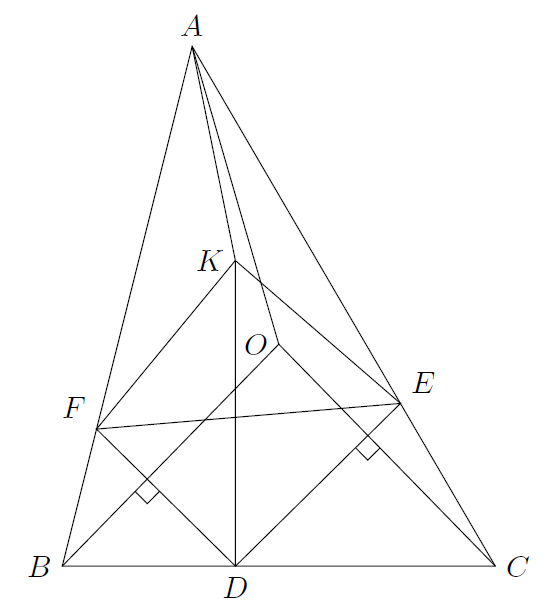
\includegraphics[width=0.3\textwidth]{seniortest2_q3.PNG}
    \end{figure}
    
    \item[4.] Let $P(x) = x^3 + \alpha x^2 + \beta x + \gamma$ where $\alpha, \beta, \gamma \in \mathbb{R}$. The condition that $P(1) = 91$ then becomes $1 + \alpha + \beta + \gamma = 91$ and $P(-1) = -121$ becomes $-1 + \alpha - \beta + \gamma = -121$. Adding the two equations yields $2 \alpha + 2 \gamma = -30$, hence $\alpha + \gamma = -15$.
    
    By Vieta's formulae, we have: $\alpha = -(a+b+c), \beta = ab + bc + ca$ and $\gamma = -abc$. Hence $abc + a + b + c = - \alpha - \gamma = 15$ and $ab+bc+ca = \beta = (1 + \alpha + \beta + \gamma) - (\alpha + \gamma) - 1 = 91 + 15 - 1 = 105$. Thus
    \[  \frac{ab+bc+ca}{abc+a+b+c} = \frac{105}{15} = 7  \]
    which is, indeed, the \textit{only} value that the fraction can attain.
    
    % EGMOE 2012 Q5
    \item[5.] Rearranging the equation, $2qn(p + 1) = (n + 2)(2pq + p + q + 1)$. The left hand side is even, so either $n + 2$ or $p + q + 1$ is even, so either $p = $2 or $q = 2$ since $p$ and $q$ are prime, or $n$ is even.
    
    If $p = 2$, $6qn = (n + 2)(5q + 3)$, so $(q - 3)(n - 10) = 36$. Considering the divisors of $36$ for which $q$ is prime, we find the possible solutions $(p, q, n)$ in this case are $(2, 5, 28)$ and $(2, 7, 19)$ (both of which satisfy the equation).
    
    If $q = 2$, $4n(p + 1) = (n + 2)(5p + 3)$, so $n = pn + 10p + 6$, a contradiction since $n < pn$, so there is no solution with $q = 2$.
    
    Finally, suppose that $n = 2k$ is even. We may suppose also that $p$ and $q$ are odd primes. The equation becomes $2kq(p + 1) = (k + 1)(2pq + p + q + 1)$. The left hand side is even and $2pq + p + q + 1$ is odd, so $k + 1$ is even, so $k = 2l + 1$ is odd. We now have
    $$ q(p + 1)(2l + 1) = (l + 1)(2pq + p + q + 1) $$
    or equivalently
    $$ lq(p + 1) = (l + 1)(pq + p + 1) $$
    Note that $q | pq + p + 1$ if and only if $q | p + 1$. Furthermore, because $(p, p + 1) = 1$ and $q$ is prime, $(p + 1, pq + p + 1) = (p + 1, pq) = (p + 1, q) > 1$ if and only if $q | p + 1$.
    
    Since $l, l+ 1)$, we see that, if $q \not | p + 1$, then $l = pq + p + 1$ and $l + 1 = q(p + 1)$, so $q = p + 2$ (and $(p, p + 2, 2(2p^2 + 6p + 3)$) satisfies the original equation). In the contrary case, suppose $p + 1 = rq$, so $l(p + 1) = (l + 1)(p + r)$, a contradiction since $l < l + 1$ and $p + 1 \leq p + r$.
    
    Thus the possible values of $q - p$ are $2, 3$ and $5$.



	
\end{enumerate}
\end{document}





